%pdflatex Fain_Masters_Thesis.tex && bibtex Fain_Masters_Thesis.aux && pdflatex Fain_Masters_Thesis.tex && pdflatex Fain_Masters_Thesis.tex

\documentclass[12pt]{tcuthesis_report}
%%%% Remove the lines below and add any custom packages or commands you need in your manuscript
\usepackage{amsmath}
\usepackage{multicol}
\usepackage{multirow}
\usepackage{url}
\usepackage{array}
\newcommand{\binocs}[0]{\textsc{binocs}\ }
\renewcommand{\thempfootnote}{\arabic{mpfootnote}}
\usepackage{siunitx}
\usepackage{xcolor}
\definecolor{AGreen}{HTML}{00ff00}
\usepackage{tikz}
\usepackage{tkz-graph}
\usetikzlibrary{automata, positioning, arrows, shapes, snakes}
\tikzset{
    ->,  % makes the edges directed
    >=stealth, % makes the arrow heads bold
    node distance=3cm, % specifies the minimum distance between two nodes. Change if necessary.
    every state/.style={thick, fill=gray!10}, % sets the properties for each ’state’ node
    initial text=$ $, % sets the text that appears on the start arrow
}

\begin{document}

%%%%% THESIS TEMPLATE INFORMATION --- Fill all of these entries in!  %%%%%%%%
\title{NEEDS A TITLE}           % Title of dissertation or thesis
\author{Baylor G.\ Fain}           % Your full name + middle initial
\hometown{Canton, Texas}     % Hometown or current city
\department{Department of Physics and Astronomy}    % TCU Department
\degreename{Masters of Science}                   % Resulting degree (MS or PHD)
\bach{Bachelor of Science, 2016\\Tarleton State University\\Stephenville, Texas}    % Description of bachelor's degree. Put line breaks before uni. name and city
\mast{} % Description of master's degree (if applicable). Format same as bachelors
\degreedate{Aug 2021}   % Expected graduation date. Month must be Dec, May or Aug
\commone{Dr.\ Hana Dobrovolny} % First member of your thesis committee (probably your advisor)
\commtwo{Dr.\ Magnus Rittby}   % Second member of your thesis committee
\commthree{Dr.\ Mia Bovill} % Third member of your thesis committee
\commfour{Dr.\ Anton Naumov}  % Fourth member of your thesis committee
\commfive{Dr.\ Ken Richardson} % Fifth member of your thesis committee
\copyright{  }          % Any necessary copyright information. Can include line breaks
\advisor{Major Advisor, Dr.\ Hana Dobrovolny, Associate Professor of Biophysics}    % Full name and title of your advisor

\frontmatter 
\acknowledgements{TextBlock/acknowledgements}  % Document which contains the text of your acknowledgements
\tableofcontents
\clearpage \listoffigures
\clearpage \listoftables
	
\mainmatter % Remove the following \input commands and change them to the files containing the text of your document
\clearpage \begin{center}
\begin{tabular}{ll}

ABM  & Agent based model\\
API  & Application Programming Interface\\
AUC  & Area under the curve\\
CUDA & Compute Unified Device Architecture\\
ET   & Eclipse time\\
HT   & Healthy time\\
IT   & Infected time\\
MDCK & Madin-Darby canine kidney\\
ODE  & Ordinary differential equation\\
PDE  & Partial differential equation\\
PDM  & Partial differential equation model\\
SSR  & Sum of square residuals\\
UT   & Universal time\\

\end{tabular}
\end{center}
 %list of abvs.
\chapter{Introduction}
%%%%%%%%%%%%%%%%%%%%%%%%%%%%%%%%%%%%%%%%%%%%%%%%%%%%%%%%%%%%%%%%%%%%%%%%%%%%%%%%%%%%
The COVID-19 pandemic, with its severity of diseases and contagability, indicates
how great of a need there is for accurate and fast modeling methods. In this thesis, I demonstrate a model that incorporates the spatial spread of viruses and produces accurate simulations in a few seconds or minutes, so that the model can be used to study viruses in a more accurate way. 

\section{Basic Virology}
Viruses are microscopic parasites, generally much smaller than bacteria, that lack the capacity to thrive and reproduce outside of a host body. A virus is composed of a nucleic acid genome and a protein capsid that covers the genome. As seen in figure \ref{fig:Virus_Replication}, the life cycle of a virus begins with the virus attaching to or being absorbed by the host cell. Once the virus genome enters into a cell, the genome moves to the ribosomes, where the genome is replicated. After the genome is replicated, new virus can be assembled and released from the host cell, allowing the virus to continue spreading through out the host cells. \citep{openstax_microbiology_2016}

\begin{figure}[h]
    \centering
    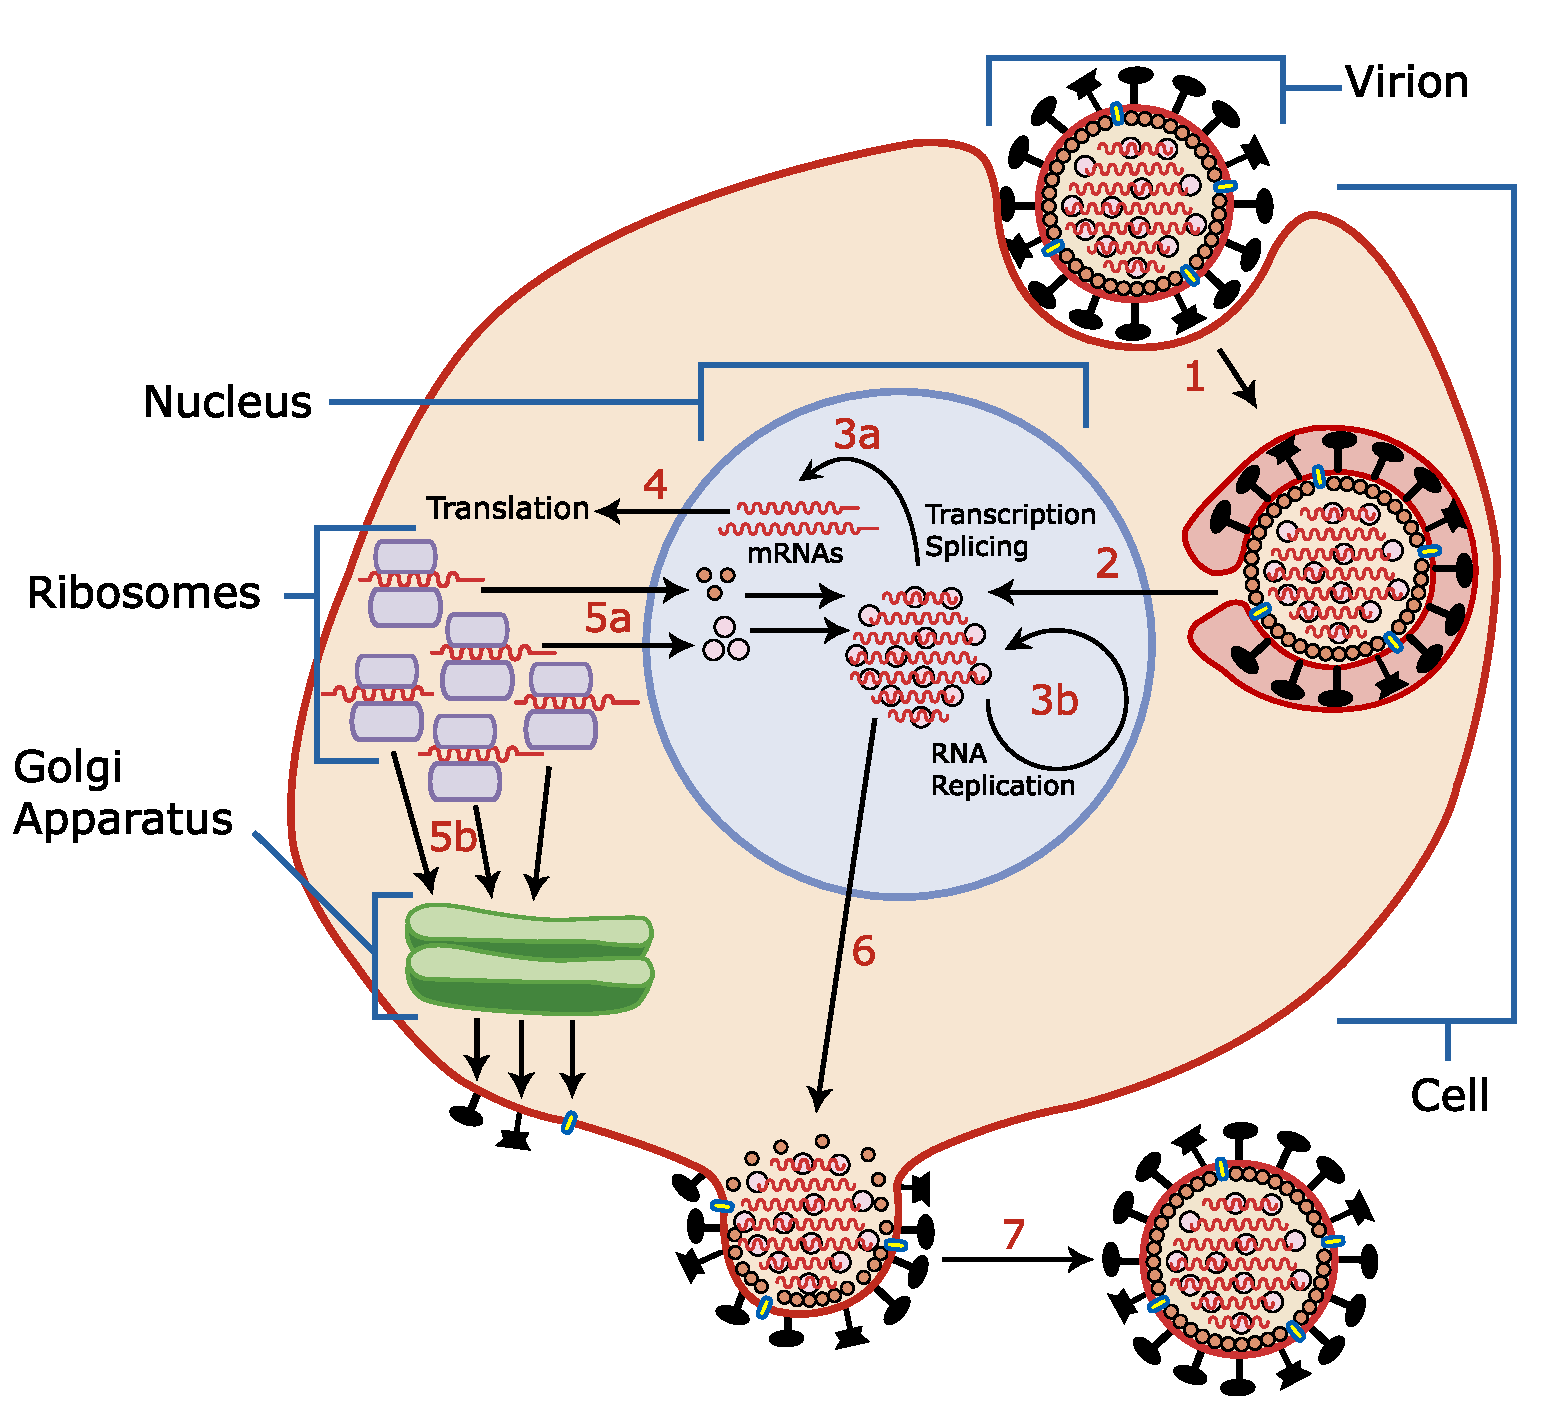
\includegraphics[width=0.6\linewidth]{Figures/Virus_Replication_large.pdf}
    \caption{The life cycle of a virus begins with a virion (virus particle) being absorbed by the cell. Once the virion enters into a cell the virus genome is released. The genome moves to the ribosomes, where the genome is replicated. With the replicated genome, new virus can be assembled by the golgi apparatus and then released from the cell.}
    \label{fig:Virus_Replication}
\end{figure}

Some viruses cause illnesses and the spread of a few has been severe enough to cause global pandemics (global outbreaks). Recent examples are the current 2019-2021 Covid-19 pandemic, the 2014 Ebola pandemic, and the 2009 Swine Flu pandemic. Other viruses are endemic (regional outbreak) or occur seasonally (yearly outbreaks), Influenza (Flu) is know for it's spread each year in the United States. In total, the Centers for Disease Control and Prevention (CDC) estimates that in the US up to 42.9 million people were sick during the 2018-2019 Flu season, 647,000 people were hospitalized, and 61,200 died. \citep{xu_update_2019}

In order to understand viruses, assays are performed. An assay is an experiment for assessing or measuring characteristics of a substance. There are two ways the assays are carried out, \emph{in vitro} or \emph{in vivo}. \emph{In vitro} are assays that are performed outside of a living organism. In virology, plaque assays are the type of  \emph{in vitro} that is most widely used for determining viral titer \citep{Kumar}.  These assays are often performed on a monolayer of cells in petri dishes or multi-well plates with a small number of wells. The dishes and plates are a type of adherent culture where the cells are grown on a nutritious substrate. The cells are grown to cover the entire surface (the point of confluence), at this point the cells tend to push on each other and distort the shape of each cell membrane \citep{bruckner_importance_2018}. Each dish/well has on the order of \numrange[range-phrase = --]{e5}{e6} cells grown on it's surface \citep{Number_of_cells_in_a_dish_noauthor_useful_nodate}. When the assay is being preformed, virus is placed in a dish/well of healthy cells. Any virus that causes damage to the cells in the dish/well can be studied. This damage is called a plaque and is roughly circular in shape. During the assay, formation of plaques and the concentration of virus are monitored. It is assumed that each plaque formed is caused by one virus particle. Because of this assumption, the viral concentration is often recorded as plaque forming units per milliliter (pfu/mL). \emph{In vivo} assays are assays that are performed in a living organism. Any virus that will infect the target animal can be studied. When the assay is being preformed virus will enter the target animal often through a nasal spray or injection. Then during the assay any visible symptoms and viral concentration are monitored.% by a nasal swab, blood test, or (as seen with mice) extraction from the lungs once the animal is sacrificed.

%%%%%%%%%%%%%%%%%%%%%%%%%%%%%%%%%%%%%%%%%%%%%%%%%%%%%%%%%%%%%%%%%%%%%%%%%%%%%%%%%%
\section{Modeling of assays}

In recent years, the field of virology has started using agent-based models to study the spread of viruses during \emph{in vitro} viral infection assays \citep{beauchemin_simple_2005,alvarado_cellular-level_2018,wodarz_laws_2014,tong_development_2015,whitman20,goyal16,itakura10,wasik14} in an effort to study the spatiality of viral spread, but currently the implementation of the agent-based models has had two issues: speed and size. The agent-based model framework is appealing to virus modelers because it allows for the individual tracking of how cells, as agents, interact with the virus, and has the potential to replicate \emph{in vitro} and eventually \emph{in vivo} viral infections. Agent-based (individual-based or micro-simulation) models have been around since 1970 with the introduction of ``Conway's Game of Life'' \citep{gardner70}. These models have been utilized in many different fields from physics to the study of fish (ichthyology) \citep{owusu20} and continue to be popularized for different applications by software like Netlogo \citep{nogare20,chiacchio14}. The models consist of a collection of agents whose behavior is determined by mathematical or computational rules. The agents of the system can move freely \citep{beauchemin07} or be fixed in a grid or lattice \citep{beauchemin_simple_2005} for varying applications, but either configuration allows for tracking of spatially emergent patterns. Agent-based models are notorious for being computationally intensive and taking long amounts of time to run simulations. This point has been commented on in a previous article \citep{gallagher_causes_2018} and the feasibility of ABMs for research has been talked about as a goal that is to come with increasing computational advancements \citep{bauer_agent-based_2009}. Previous research has addressed this lack of computing power issue by reducing the number of agents modeled and therefore reducing the number of computations required for a simulation. The number of agents published is at minimum an order of magnitude lower then the number of target cells used in the corresponding experimental data. Beauchemin et al.\ \citep{beauchemin_simple_2005} simulated \num{1.232e5} agents, while the experiment they were attempting to replicate was performed in 6 well-plates and had $\sim$\num{1.2e6} cells per well. Alvarado et al.\ \citep{alvarado_cellular-level_2018} simulated \num{4.0e4} agents when trying to replicate experiments also performed in 6 well-plates. Wodarz et al.\ \citep{wodarz_laws_2014} simulated \num{2.0e4} agents, while the experiment they were replicating was performed in 24 well-plates and had $\sim$\num{2.4e5} cells per well. Tong et al.\ \citep{tong_development_2015} simulated \num{6.0e5} agents in an effort to simulate mice lungs, which have $\sim$\num{e9} cells. These smaller simulations are more affected by boundary interactions, which can result in model dynamics that don't faithfully reproduce the infection. Having an in-host model that can produce accurate simulations in a timely manner not only allows for the prediction of patient infection, but also can be used to flush out potential causes of varying symptoms in patients. 

%%%%%%%%%%%%%%%%%%%%%%%%%%%%%%%%%%%%%%%%%%%%%%%%%%%%%%%%%%%%%%%%%%%%%%%%%%%%%%%%%%
\section{Exigence}
While it might be feasible to wait long periods of time to run accurate simulations for endemic or recurrent seasonal viruses, recent events of the COVID-19 pandemic indicate how great a need there is for accurate and fast modeling methods. Epidemiological population-level modeling tools that include both ordinary differential equation (ODE) models \citep{li20,ngonghala20} and ABMs \citep{ying21,sneppen21,kano21} were immediately deployed to help predict how the new virus would spread around the world and how different interventions could help stem the spread. At the within-host level, the primary modeling tool was limited to simple ODE models \citep{goncalves20,wang20model,hernandez20,dogra20} that lack the ability to reproduce the spatial heterogeneity of real viral infections. Fast and accurate in-host models could be helpful in assessing the potential of re-purposed drugs \citep{czuppon21,goncalves20,dodds20}, finding indicators of disease severity or mortality \citep{neant21}, and assessing the effectiveness of testing \citep{ejima21}. A community-driven ABM incorporating many realistic biological responses was quickly developed for SARS-CoV-2 \citep{getz21}, but is only currently simulating a few thousand agents and is expected to need high-performance computing or cloud resources to parameterize the model. Thus, there is a need to develop modeling and simulation tools for accurately predicting in-host viral dynamics that can be quickly deployed to help combat the next pandemic.

%%%%%%%%%%%%%%%%%%%%%%%%%%%%%%%%%%%%%%%%%%%%%%%%%%%%%%%%%%%%%%%%%%%%%%%%%%%%%%%%%
\section{Scope}

In this work, the testing, validation, and application of a hybrid ABM and partial differential equation model (PDM) implemented on GPUs is presented. The work here begins with the methods where the four attributes of the model: (1) the agent-based model of the cells, (2) the partial differential equation of the virus, (3) the cell-free transmission mode of viruses, and (4) fitting of the model to data, are explained.  Then, the results of model implementation with parallel programming, convergence testing, and simulation speed improvement are presented. Finally, I show that the model can reproduce experiments by fitting the model to an \emph{in vitro} influenza virus experiment and an \emph{in vitro} SARS-Cov-2 experiment. This work shows how an ABM/PDM hybrid model of in-host infections is ensured to numerically converge, be applied to experimental data for parameter extraction, and produce simulations with in seconds to minutes for timely application.





\chapter{Model Validation and Calibration}
When studying something like viruses, that can have a huge effect on a person let alone a society, it is crucial to produce accurate simulations quickly. In the previous chapter, I showed how the field of virology has tried to use ABMs to capture the spatial spread of viruses, but does not have either the computing power or coding tools to make the ABMs feasible. In this chapter, a model for studying virus that incorporates the physics of viral spread both quickly and accurately is given in detail. I will present how the model accounts for spatial spread of virus, is able to produce simulations without compromising on accuracy, and can be applied to real experimental data. 

\section{Model details}

In this work, a two dimensional biological system is simulated with a mathematical model. The system is a culture dish of a monolayer of cells with virus diffusing over the cells. The model is a hybrid of an agent based model (ABM) and a partial differential equation model (PDM) where the cells are represented with an ABM and the virus diffusion is represented by a PDM.

\subsection{Spatial accounting} \label{Spatial_accounting}

To allow for the two dimensional aspect of the culture dish to be represented in the model, the cells are approximated as hexagons. Using hexagons enables for an elegant managing of the cells' shapes in the dish and the viral transmission. Since the culture dishes are grown to confluence, the cells are close enough that they push on each other and the cell walls deform. This causes the cells to no longer be in the shape of a circle, but become irregular polygons with multiple sides \citep{bruckner_importance_2018}. Modeling the cells as hexagons gives the cells definite sides and the cells are able to span any two dimensional region forming a hexagonal grid. Furthermore, by using a hexagonal grid, when virus particles spread among this population of cells the indexing of the grid can be used to find the neighbors of any cell. This will be used for cell-free transmission to know where virus will flow away from (high concentrations areas) and to (low concentration areas) during diffusion. In addition to helping with the physical representation of the model, hexagonal coordinates have some other attributes that can be utilized to optimize the code for quicker compute times. The three attributes that this code utilizes are:
\begin{enumerate} 
    \item The coordinates can be split in to three sectors where the coordinates $X_{hex}$, $Y_{hex}$, and $Z_{hex}$ are simply cyclic permutations.
    \item The $X_{hex}$ and $Z_{hex}$ directions can be used as indices of a matrix.
    \item The coordinates of the neighboring hexagons are found by adding a cyclic permutation of 
        $\left [
            \begin{array}{c}
                1 \\
                0 \\
                -1\\
            \end{array}
        \right ]$
        for three of the neighbors and
        $\left [ 
            \begin{array}{c}
                1 \\
                -1 \\
                0\\
            \end{array}
        \right ]$
        for the other three neighbors.
\end{enumerate}
These attributes save time by either reducing the number of calculations needed or the amount of searching through data arrays. Attribute 1 allows for only a third of the cell locations to be calculated and Attributes 2 and 3 give the data a reference so that adjacent data in memory can be found quicker.

\subsection{Agent-based model} \label{ABM}

In an ABM, a system is broken down into smaller units called ``agents''. Each of the agents are governed by a set of rules on a local scale with large scale phenomena resulting from interaction of the agents, so the two scales are studied to find the connections. As a simulation of the model is stepped through time, the agents act and interact. These actions cause bulk properties, that may appear disconnected from the individual agents, to manifest. Properties are observed and measured to find the connection between the small interactions and large scale properties.

In this work, an ABM governs the transitions a cell makes through the stages of infection: healthy, eclipse, infected, and dead. A cell in the healthy state is an uninfected cell that remains healthy until infected. A cell in the eclipse state is an infected cell that is not yet producing virus. The cell remains in the eclipse state for an average amount of time, $\tau_E$. The specific time value for each cell is determined by a gamma distribution with shape value $\eta_E$ and scale value $\tau_E/\eta_E$. A cell in the infected state is an infected cell that is producing virus. The cell remains in the infected state for an average amount of time, $\tau_I$. The specific time value for each cell is determined by a gamma distribution with shape value $\eta_I$ and scale value $\tau_I/\eta_I$. A gamma (Erlang) distribution is used for the amount of time in the eclipse and infected phase, as suggested by the work of Beauchemin et al.\ \citep{beauchemin17} and Kakizoe et al.\ \citep{kakizoe15}. A cell in the dead state is a cell that can no longer change state, so once a cell is in the dead state the cell remains in that state until the end of the simulation. The flow of this is illustrated in figure \ref{fig:transitioning_through_the_stages_of_infection}.

The ABM uses four time arrays to track and transition the cells to different states after infection. The four arrays universal time (UT), healthy time (HT), eclipse time (ET), and infected time (IT) have an element for each cell. The universal time array holds the amount of time that each cell has been in the simulation; each element starts at zero and increases each iteration by the simulation's time step. The healthy time array holds the amount of time that a cell is healthy; each element starts at zero and while the cell is healthy increases each iteration by the simulation's time step. The eclipse time array holds the amount of time each cell is in the eclipse state and the infected time array holds the amount of time each cell is in the infected state. For the eclipse and infected arrays the amount of time is fixed and the value is determined by a gamma (Erlang) distribution, as described above. The flow of this is illustrated in figure \ref{fig:transitioning_through_the_stages_of_infection}.

%\begin{figure}
%    \centering
%    \begin{tikzpicture}[state/.style={regular polygon,regular polygon sides=6, draw, minimum size=2.5cm, inner sep=0pt, outer sep=0pt}]
%    \node[state, draw=AGreen, fill=AGreen!10] (H) {$Healthy$};
%    \node[state, draw=cyan, fill=cyan!10, right of=H] (E) {$Eclipse$};
%    \node[state, draw=red, fill=red!10, right of=E] (I) {$Infected$};
%    \node[state, draw=black, fill=black!10, accepting, right of=I] (D) {$Dead$};
%    
%    \draw   (H) edge[bend left=45] node [above] {} (E);
%    \draw   (E) edge[bend left=45] node [above] {$\tau_E$} (I);
%    \draw   (I) edge[bend left=45] node [above] {$\tau_I$} (D);
%    \end{tikzpicture}
%    \caption{The stages of infection healthy, eclipse, infected, and dead are shown. Cells stay in  the eclipse stage for an average time $\tau_E$ and in the infected stage for an average time $\tau_I$.}
%    \label{fig:stages_of_infection}
%\end{figure}

%\begin{figure}
%    \centering
%    \begin{tikzpicture}[state/.style={regular polygon,regular polygon sides=6, draw, minimum size=2.5cm, inner sep=0pt, outer sep=0pt}]
%        \node[state, draw=AGreen, fill=AGreen!10] (H) {$Healthy$};
%        \node[state, draw=cyan, fill=cyan!10, below right of=H] (E) {$Eclipse$};
%        \node[state, draw=red, fill=red!10, below right of=E] (I) {$Infected$};
%        \node[state, draw=black, fill=black!10, accepting, below right of=I] (D) {$Dead$};
%            
%        \draw   (H) edge[bend left=45] node [above right] {Infection event} (E);
%        \draw   (E) edge[bend left=45] node [above right] {UT $>$ HT + ET} (I);
%        \draw   (I) edge[bend left=45] node [above right] {UT $>$ HT + ET + IT} (D);
%    \end{tikzpicture}
%    \caption{Transitioning through the stages of infection: UT is the universal time for a cell, HT is the healthy time for a cell, ET is the eclipse time for a cell, and IT is the infected time for a cell.}
%    \label{fig:transitioning_through_the_stages_of_infection}
%\end{figure}

\begin{figure}
    \centering
    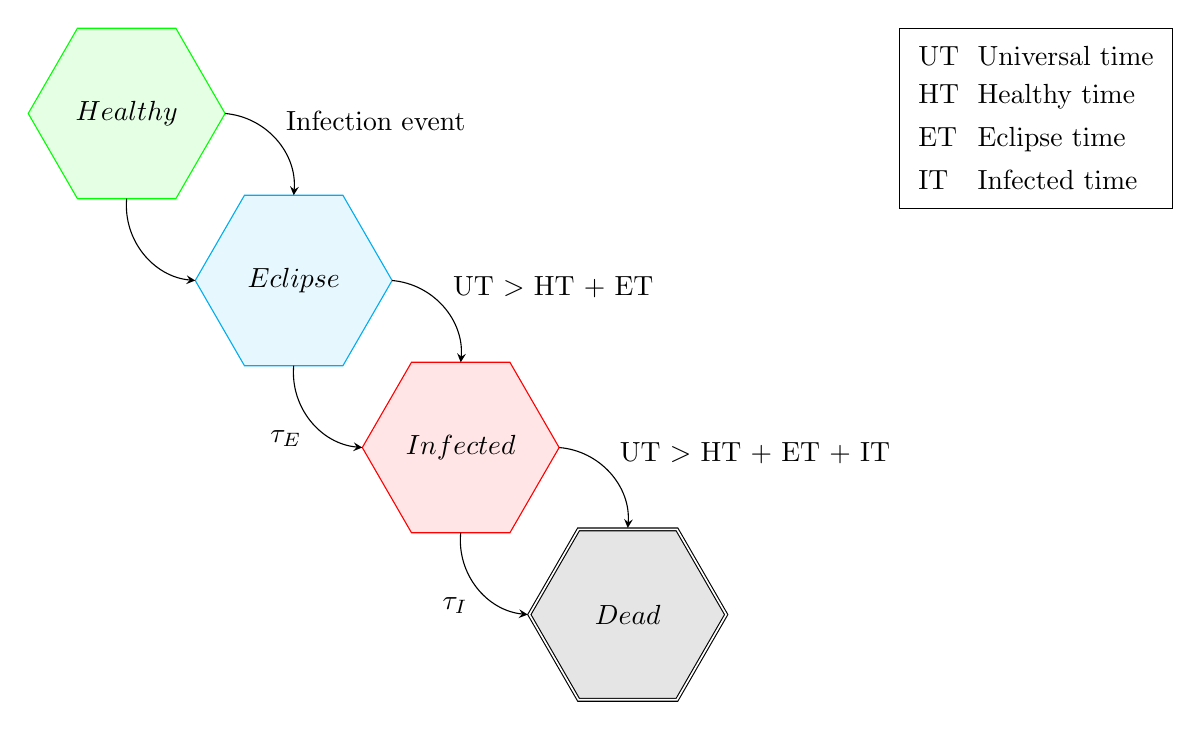
\begin{tikzpicture}[
        Healthy/.style={regular polygon,regular polygon sides=6, draw, minimum size=2.5cm, inner sep=0pt, outer sep=0pt, draw=AGreen, fill=AGreen!10},
        Eclipse/.style={regular polygon,regular polygon sides=6, draw, minimum size=2.5cm, inner sep=0pt, outer sep=0pt, draw=cyan, fill=cyan!10},
        Infected/.style={regular polygon,regular polygon sides=6, draw, minimum size=2.5cm, inner sep=0pt, outer sep=0pt, draw=red, fill=red!10},
        Dead/.style={regular polygon,regular polygon sides=6, draw, minimum size=2.5cm, inner sep=0pt, outer sep=0pt, draw=black, fill=black!10}]

        \node[Healthy] (H) {$Healthy$};
        \node[Eclipse, below right of=H] (E) {$Eclipse$};
        \node[Infected, below right of=E] (I) {$Infected$};
        \node[Dead, accepting, below right of=I] (D) {$Dead$};
            
        \draw   (H) edge[bend left=45] node [above right] {Infection event} (E);
        \draw   (E) edge[bend left=45] node [above right] {UT $>$ HT + ET} (I);
        \draw   (I) edge[bend left=45] node [above right] {UT $>$ HT + ET + IT} (D);

        \draw   (H) edge[bend right=45] node [below left] {} (E);
        \draw   (E) edge[bend right=45] node [below left] {$\tau_E$} (I);
        \draw   (I) edge[bend right=45] node [below left] {$\tau_I$} (D);

        %Legand with text
        \matrix [draw,
                below right,
                column 1/.style={anchor=base west},
                column 2/.style={anchor=base west}
                ] at (current bounding box.north east) 
        {
          \node [] {UT}; & \node [] {Universal time}; \\ 
          \node [] {HT}; & \node [] {Healthy time}; \\ 
          \node [] {ET}; & \node [] {Eclipse time}; \\ 
          \node [] {IT}; & \node [] {Infected time}; \\ 
        };

%        %Legand with nodes
%        \matrix [draw, below left] at (current bounding box.north east) {
%          \node [Healthy, scale=0.3, label=right:Healthy] {}; \\
%          \node [Eclipse, scale=0.3, label=right:Eclipse] {}; \\
%          \node [Infected, scale=0.3, label=right:Infected] {}; \\
%          \node [Dead, scale=0.3, label=right:Dead] {}; \\
%        };
    \end{tikzpicture}
\caption{The stages of infection: healthy, eclipse, infected, and dead are shown. The cells transition through the stages at different time points. Above: The time point when a state transition occurs is shown in terms of UT, the universal time, for a cell. Below: The time point when a state transition occurs is shown in terms of average time. $\tau_E$ is the average time a cell stays in  the eclipse stage and $\tau_I$ is the average time a cell stays in the infected stage. UT is the time a cell has existed, HT is the time a cell has been healthy, ET is the time a cell is in the eclipse phase, and IT is the time a cell is in the infected phase. \label{fig:transitioning_through_the_stages_of_infection}}
\end{figure}

\subsection{Partial differential equation model} \label{PDM}

PDMs are used to model multiple dimensions; in this work a PDE in hexagonal coordinates is used to model the two-dimensional spatial spread of virus over cells in a culture dish. In a PDM, the dynamics of a system can be represented by a partial differential equation, or more specifically, an equation that contains multi-variable functions that represent important system aspects and one or more partial derivatives of those functions. In the culture dish, as an infected cell releases virus into the extracellular fluid, the virus diffuses across a density gradient. The PDM represents this diffusion with the diffusion equation, 
\begin{equation}
\frac{\partial V}{\partial t}=D \nabla^{2}V + p - cV, \label{diff_eq}
\end{equation}
where $V$ is the density of the virus, $D$ the diffusion coefficient, $p$ is the production rate per cell, $c$ is the viral clearance rate. In the code, along with the assumption of hexagonal cells, the cells are assumed to be flat, so the virus is diffusing over a smooth two dimensional plane. This assumption allows for the use of the two dimensional diffusion equation in hexagonal coordinates, so Eq.\ \eqref{diff_eq} becomes 
$$\frac{\partial V}{\partial t} = D\frac{2}{3} \left (\frac{\partial^2}{\partial x^2_1}+\frac{\partial^2}{\partial x^2_2}+\frac{\partial^2}{\partial x^2_3}\right )V + p -cV$$ 
where  
$\textbf{x}_1=
\left [
    \begin{array}{c}
        1 \\
        0 \\
    \end{array}
\right ]$, 
$\textbf{x}_2=
\left [
    \begin{array}{c}
        -1/2 \\
        \sqrt{3}/2 \\
    \end{array}
\right ]$, and 
$\textbf{x}_3=
\left [
    \begin{array}{c}
        -1/2 \\
        -\sqrt{3}/2 \\
    \end{array}
\right ]$ 

are the unit vectors for a hexagonal grid. For computation, a forward Euler implementation of the PDM with Neumann boundary conditions is used.

\subsection{Viral transmission} \label{Viral_transmission}

When a virus is spreading among the cells in a culture dish, there is a probability that a healthy cell becomes infected by virus that is not within a cell, but flowing around and above the cell. When this viral transmission occurs it is called cell-free transmission. For cell-free transmission, the probability per unit time ($\mathrm{P_{cf}}$) that a cell becomes infected is determined by the amount of virus that is covering the cell ($V$) times the infection rate ($\beta$) \citep{holder11autoimm}, 
$$\mathrm{P_{cf}} = V \beta.$$ 
As a healthy cell becomes surrounded by more virus, the probability of cell-free infection increases. If the probability ($V \beta \Delta t$) is ever greater than one due to the build up of virus, an adaptive time step is used. The time step ($\Delta t$) is divided in half repeatedly until the probability of cell-free infection is below one. Once the probability is finalized, a number from the uniform distribution is compared with the probability of cell-free infection. If that number is less than $\mathrm{P_{cf}}$, then the cell becomes infected.

%1 - y = (1-m)^n

\subsection{Parameters of viral spread}

The eight parameters $\beta$, $\tau_E$, $\eta_E$, $\tau_I$, $\eta_I$, $p$, $c$, and $D$ affect the dynamics of virus spread in the model. Four of the parameters, $\tau_E$, $\eta_E$, $\tau_I$, and $\eta_I$, are used in the ABM to choose the time duration that a cell is in the eclipse and infected phase as mentioned in section \ref{ABM}. Three of the other parameters, $p$, $c$, and $D$, are used in the PDM and characterize the differential equation, as mentioned in section \ref{PDM}. The final parameter, $\beta$, governs the interaction between the virus and cells, setting the probability that the cell is infected. In order to model a particular virus, values for these parameters need to be chosen. The initial values of the parameters are chosen from ordinary differential equation models of influenza and listed in Table \ref{tab_params} (viral titer units have been converted to virions, as described in \citep{dobrovolny17}). %For $\eta_E$, $\eta_I$, $c$, and $D$ the values are fixed, but for $\beta$, $\tau_E$, $\tau_I$, and $p$ the values serve as a starting point for the model to be fit to real experimental data.

\begin{table}
%\centering
\caption{Parameter values to simulate an influenza infection with the ABM/PDM model.\label{tab_params}}
\resizebox{\textwidth}{!}{%
\begin{tabular}{llcr}
\hline
Parameter & Meaning & Value & Reference\\
\hline
$\beta$ & Infection rate & 2.0 $/\mathrm{h}$ & Scaled from Beauchemin et al.\ \citep{beauchemin08}\\
$p$ & Viral production rate & 562800 $/\mathrm{h}$ & Scaled from Beauchemin et al.\ \citep{beauchemin08}\\
$c$ & Viral clearance rate & 0.105 $/\mathrm{h}$ & Beauchemin et al.\ \citep{beauchemin08}\\
$D$ & Diffusion coefficient & 2.16$\times 10^{-8}$ $\mathrm{m}^2/\mathrm{h}$ & Stokes-Einstein equation\\
$\tau_E$ & Mean eclipse duration & 6.0 $\mathrm{h}$ & Beauchemin et al.\ \citep{beauchemin08}\\
$\eta_E$ & Eclipse shape parameter & 30 & Pinilla et al.\ \citep{pinilla12}\\
$\tau_I$ & Mean infectious lifespan & 12.0 $\mathrm{h}$ & Beauchemin et al.\ \citep{beauchemin08}\\
$\eta_I$ & Infectious shape parameter & 100 & Pinilla et al.\ \citep{pinilla12}\\
\end{tabular}}
\end{table}

%In order to determine which parameter values minimize the SSR, a brute force walk of a parameter space is performed. The axes of the parameter space are four arrays that are constructed around the initial values of $\beta$, $p$, $\tau_I$, and $\tau_E$, shown in Table \ref{tab_params}. Two values, increasing or decreasing by 25\%, are added on both sides of the initial points; resulting in a total of 5 points per array and 625 points total in the parameter space.

\section{Computational details}

In this work, the simulations are of viral infections, that can have drastic effects on those infected, so the model needs to produce simulations that are fast, numerically sound, and have realistic results. The model uses parallel processing on GPUs to reduce simulation times without reducing complexity. Additionally, the simulations are tested for numerical convergence and are then fit to real experimental data in order to reproduce experiments.

\subsection{Implementation on GPUs}

As the model becomes more complex, GPU acceleration via parallel programming is used to decrease the simulation run times and therefore increase the number of studies that can be conducted in a given time. In the simulations, the cells change state based on the amount of virus above them. The number of cells in a culture dish is on the order of $10^6$ cells \citep{Number_of_cells_in_a_dish_noauthor_useful_nodate}, so the ABM will simulate a grid of $1001365$ agents of hexagonal cells in a circle to best replicate what is happening in the experiment. Each agent will follow the rules of checking the amount of virus above the cell every time step. Utilizing attribute 2 of hexagonal coordinates from section \label{Spatial_accounting}, the number of calculations is reduced from the order of ($\mathcal{O}(n^2)$) per time step to the order of the number of agents ($\mathcal{O}(n)$). The calculations from the agents' rules are split over the processing units of a GPU to be calculated in parallel or simultaneously. To utilize this processing, Nvidia's CUDA (Compute Unified Device Architecture) is used to implement the ABM and PDM. CUDA is an Application Programming Interface (API) that allows the many processing units (cores) on a Nvidia brand GPU to be used for computing. %The ability to manipulate what is happening at the cellular level of the simulations allows for generation of isolated studies of the viral transmission. The isolated studies of how cells are infected are analyzed and the characteristics from section \ref{Viral_transmission} are compare to find any trends in the data



%%%%%%%%%%%%%%%%%%%%%%%%%%%%%%%%%%%%%%%%%%%%%%%%%%%%%%%%%%%%%%%%%%%%%%%%%%%%%%%%%%
\subsection{Convergence Testing} \label{methods_convergance}

Partial differential equations (PDEs) are a popular way to model systems that evolve over both space and time, but often require computers to produce solutions. With PDEs, even systems that have an exact solution often need to be calculated on a computer because of the infinite series that are required in those solutions. Therefore, solutions to PDEs are often found through numerical integration. In the numerical integration, space and time are assumed to be made up of small units or discretized. From this discretization, time is a one dimensional line of points separated by a chunk of time called $\Delta t$ and two dimensional Cartesian space is a grid with a line of points for each dimension where there is a chunk of space for each dimension $\Delta x$, $\Delta y$. At these points in time and space, a numerical integration scheme approximates the solution of the PDE. Different numerical schemes have different benefits. Depending on the phenomena that needs to be studied with the PDE the size of $\Delta t$, $\Delta x$, and $\Delta y$ and the choice of numerical scheme are important. If the chunks of space or time are too large then the simulation does not have the resolution to resolve phenomena that occur at smaller increments in the model and if the numerical scheme requires to much computing power then the solutions can not be found in a timely manner.

Depending on the choice of numerical scheme, a conditional relationship between $\Delta t$, $\Delta x$, and $\Delta y$ must be met. For the symmetric, two dimensional Euler's method $$ \Delta t \leq \frac{(\Delta x)^{2}}{4 D},$$ is the conditional relationship \citep{wendroff_difference_1968,olsen-kettle_numerical_nodate}. Satisfying this relationship is necessary to ensure that the sequence of approximations that the numerical scheme uses to approximate a solution converges, otherwise the error grows exponentially to a point that the solutions are unreliable. Using the relationship above, values for $\Delta t$, $\Delta x$, and $\Delta y$ can be chosen to ensure stability of the error in the numerical scheme. As long as that relationship is met the solution is reliable within a certain error, but the relationship does not give the $\Delta t$, $\Delta x$, and $\Delta y$ that are best for producing accurate simulations with the least amount of computing cost.

To ensure the simulations are not using more resources than necessary, the space and time discretizations: $\Delta t$, $\Delta x$, and $\Delta y$ need to be optimized. Convergence testing is a simple brute force method where the input parameters are increased or decreased by a particular amount and the accuracy or trends of the simulation are measured for each of the the new increments. Schemes for convergence testing are implemented and studied in fields like computational fluid dynamics \citep{bermejo16,kim20fluid} and astrophysics \citep{xu21,banei21}. The model proposed in this work has fixed $\Delta x$ and $\Delta y$, because the simulations are of real cells, whose average diameter can be measured between \numrange[range-phrase = --]{50}{100} \si{\micro\meter}. \color{red} What is cell size set to in your implementation? \color{black} Thus the convergence testing only has to be conducted for $\Delta t$. To conduct the study a starting point of 0.005 hr, about 5.78 times smaller than the conditional relationship, was chosen and a range of seven values was created by multiplying or dividing the initial $\Delta t$ by 2 repeatedly. For each of these $\Delta t$s, the median viral titer curve of ten simulations were compared.

\subsection{Measurements} \label{convergence_measures}

As the viral infection progresses the total amount of virus in the culture dish changes and the shape of the total amount of virus over time can change depending on the virus being use for the infection. Plotting the amount of virus vs.\ time produces a curve that has a distinct shape and has characteristics that can be measured. The measurements, shown in Figure \ref{measurements} and defined below, can be used to compare multiple viruses or to compare multiple simulations of the same virus with different input parameters. In this thesis, I will use them to verify the convergence of the simulation.
\begin{itemize}
\item \textbf{peak viral load:} The maximum amount of virus is commonly used as an indicator of the transmissibility of an infection \citep{handel09}. 
\item \textbf{time of viral peak:} This is the time between the start of the infection and the peak of the virus and can give an indication of how quickly the virus is replicating.
\item \textbf{viral upslope:} Viral upslope is the exponential growth rate of the viral titer before the peak is reached and is another indication of how quickly the virus is spreading from cell to cell. 
\item \textbf{viral downslope:} Viral downslope is the exponential decay rate of the viral titer after the peak. While the slope during the decay phase is negative, we define downslope as the positive value of the slope.
\item \textbf{area under the curve (AUC):} AUC is often used to assess the severity of an infection \citep{hayden00, barroso05}.
\item \textbf{infection duration:} The infection duration is indicative of how long an infected patient might test positive for presence of the virus. In this work $10^1$ virions is the threshold.
\end{itemize}

\begin{figure}
\begin{center}
    \resizebox{0.6\textwidth}{!}{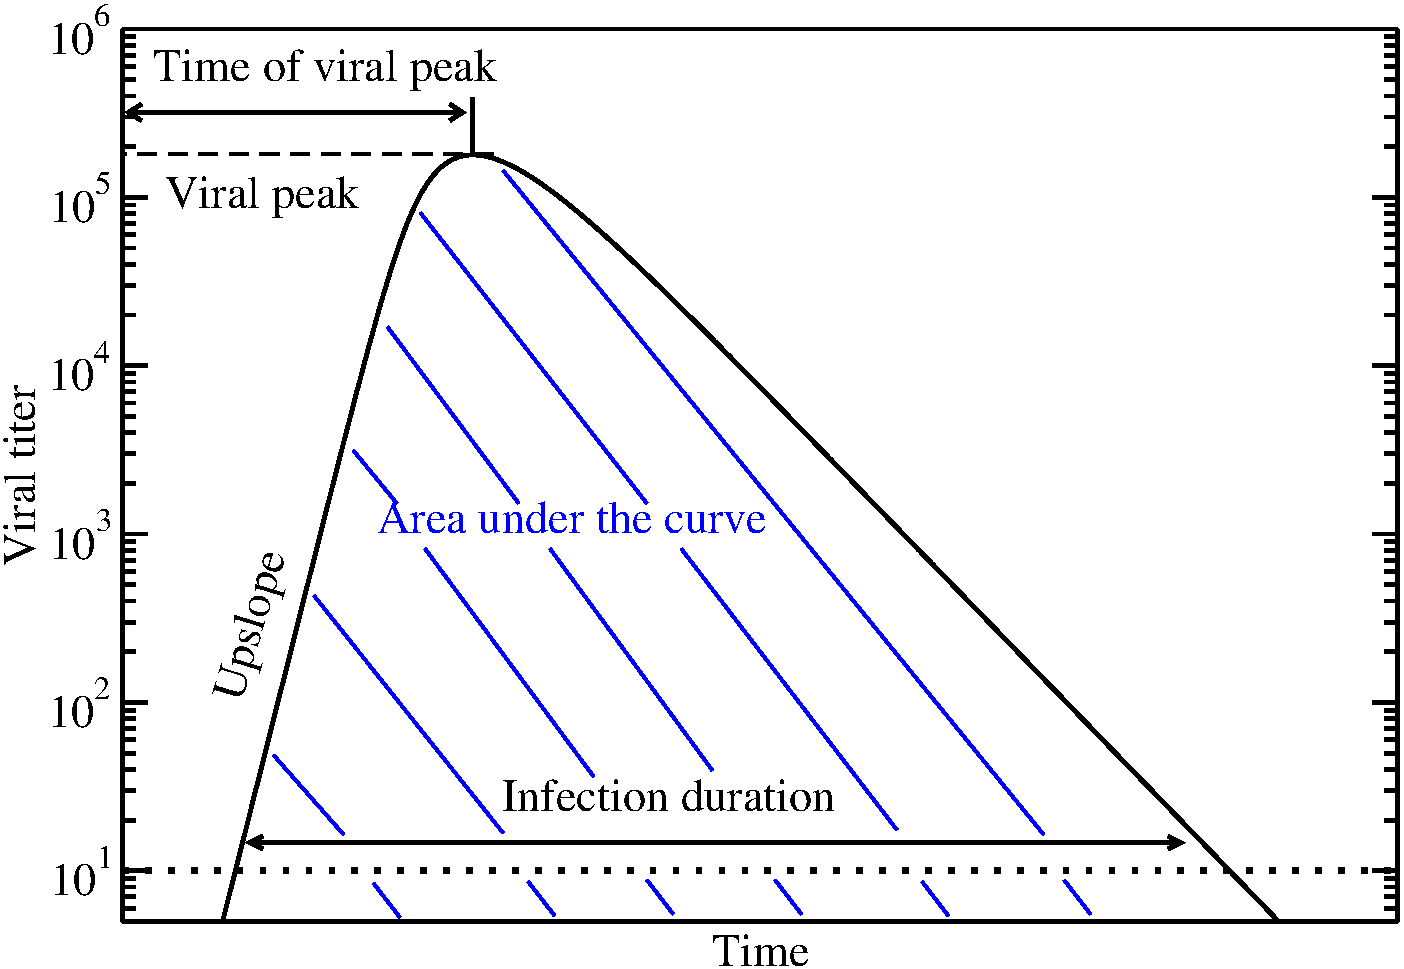
\includegraphics{Figures/measurements.pdf}}
    \caption{Measurable characteristics of the viral titer curve.}
    \label{measurements}
\end{center}
\end{figure}


\section{Data Fitting} \label{Data_Fitting}

As part of our model validation, the model is tested to ensure it can reproduce viral titer curves observed experimentally. We use three experimental data sets varying both virus and cell type. The first data set used here is from an \emph{in vitro} experiment performed by Pinilla et al.\ \citep{pinilla12}. During the study, a well of a 24-well plate, containing Madin-Darby canine kidney (MDCK$\alpha$2,6) cells was inoculated with the A/Qu\'{e}bec/144147/09 (H1N1) pandemic strain of influenza virus and the supernatant fluid was collected every 6 hours until 36 hours and then every 12 hours until 72 hours post infection. The supernatant was then used for RNA isolation and/or viral titration by standard plaque assay on MDCK$\alpha$2,6 cells. The specific data referenced for this work is the ``Multiple-cycle viral yield" experiment shown in figure 2A of the Pinilla et al.\ manuscript. 

The second and third data sets are from an \emph{in vitro} experiment performed by \cite{wang_susceptibility_2021}. During the study, 25 cell lines where inoculated with \num{5e4} TCID$_{50}$ per well of  SARS-CoV-2/USA-WA1/2020 (USA-WA1). The Vero and Vero76 cell line data will be used here for the fitting process. The supernatant fluid was recorded initially at 0 hours and washed away at 2 hours. Supernatent was then collected every 24 hours until 120 hours post infection. The supernatant was used for viral RNA quantification. The specific data referenced for this work is the Vero cell lines and the Vero76 cell lines of the ``Replication of SARS-CoV-2 in a Large Set of Cell Substrates" experiment shown in figure 2 of the Wang et al.\ manuscript. Data was extracted from both manuscripts using WebPlotDigitizer (https://automeris.io/WebPlotDigitizer/). 

To determine the best fit of the model to the experimental data, the sum of square residuals (SSR) is minimized, $$\mathrm{SSR} = \sum_{i=1}^{n} (y_i - \hat y_i)^{2},$$ where $y_i$ is from the experimental data set and $\hat y_i$ is from the simulated data set. In our case, the simulated data set is the average of ten cell-free transmission simulations. The initial conditions for the simulations are: Total cells -- $1001365$, Total virus -- $0.0$, and MOI -- $5\times 10^{-5}$. To perform the minimization, a separate code that utilizes the function \texttt{minimize} from the python package \texttt{scipy}, was written. In the code, five parameters ($\beta$, $p$, $\tau_I$, $\tau_E$, and $c$) are allowed to vary and the remaining parameters are held fixed to the values given in Table \ref{tab_params}. The minimization code is given an initial guess for the five parameters, then by the Nelder-Mead method the next set of parameters is produced, until the minimum SSR is found.
%%%%%%%%%%%%%%%%%%%%%%%%%%%%%%%%%%%%%%%%%%%%%%%%%%%%%%%%%%%%%%%%%%%%%%%%%%%%%%%%%%%

\section{Summary}

In this chapter, I've described the construction of a hybrid ABM/PDM model of viral infections and I've outlined the techniques that will be used to test the reliability and validity of the model. 

\chapter{Model Application}
\section{Introduction}

The novel coronavirus, SARS-CoV-2, originated in Wuhan, China in late 2019 and rapidly spread around the world \citep{chen20,wu20}. This virus causes the Covid-19 disease which can lead to severe illness needing long hospitalization \citep{sun20,goyal20,jiang20}, but at the same time a significant fraction of those who contract the virus experience an asymptomatic Covid-19 disease \citep{he20}. It is still not entirely clear who is at risk for developing severe disease, although correlations of disease severity with levels of vitamin D \citep{ilie20}, levels of various immune components \citep{liu20imm,liu20imm2,zhang20imm,yang20imm}, and age \citep{borghesi20,zhang20imm} have been noted. There has also been investigation of the possibility of disease severity being linked to initial viral inoculum \citep{little20, guallar20, ghandi20}.

The major route of transmission for SARS-CoV-2 is airborne droplets \citep{morawska20}. One study indicates that sneezing and coughing creates a turbulent gas cloud that can cause viral-laden droplets to spread up to 27 feet (\numrange[range-phrase = --]{7}{8}\si{\meter}) \citep{bourouiba20}, and allows the virus to get into the ventilation system of a building. A review of literature on droplet and airborne viral spread concludes that 8 of 10 studies showed that droplets spread further than the 6 foot \citep{bahl20} social distancing recommendation. While personal protective equipment is helpful in reducing the ability of virus to enter the respiratory tract, it is not perfect \citep{mittal20}. All of these factors lead to exposures to vastly different quantities of virus when people are going about their daily activities. Thus it is important to understand whether different initial inocula lead to different viral dynamics in patients. 

There is some evidence from other respiratory viruses that the size of the initial inoculum could play a role in the severity of the illness. An influenza epidemiological modeling study suggests that a higher initial dose can lead to a higher mortality rate \citep{paulo10}. This is corroborated by an influenza in-host modeling study that also finds a correlation between the initial viral dose and survival rate \citep{price15}. Other modeling studies have found dependence of other measures of infection severity on initial dose for influenza \citep{moore20}, respiratory syncytial virus \citep{wethington19}, adenovirus \citep{li14}, and porcine reproductive and respiratory virus \citep{go19}. There are also experimental studies that find a link between dose and infection severity. Experiments using influenza have found inoculum dose dependence of total number of infected cells and area under the curve \citep{manicassamy10}, peak viral titer \citep{ginsberg52,iida63,ottolini05}, viral growth rate \citep{ginsberg52}, and time of viral peak \citep{iida63,ginsberg52}. Experiments with other viruses, such as adenovirus \citep{prince93}, and parainfluenza \citep{ottolini96}, have also shown correlations between initial inoculum and various measures of disease severity. If SARS-CoV-2 shows a similar pattern, initial inoculum should be considered as a possible contributor to infection severity and adverse outcomes.

\subsection{Mathematical model}

We use an ABM to model transitions of cells as they go through the infection cycle. We use a hexagonal grid and simulate 10$^6$ cells in a circular dish to mimic an in vitro system. Cells begin as healthy target cells that can be infected by viruses that are sitting above them. Once infected, the cells move into an eclipse phase where they are not yet actively producing virus. The cells remain in the eclipse phase for a time chosen from an Erlang distribution with mean time $\tau_E$ and shape parameter $n_E$. The cells then pass into the infectious phase, where they are actively producing virus, for a time chosen from an Erlang distribution with mean time $\tau_I$ and shape $n_I$, after which time the cells die and no longer participate in the infection. Erlang distributions are used for both transitions based on experiments that show the time spent in the eclipse phase and the time spent in the infectious phase are best described by Erlang distributions \citep{kakizoe15, beauchemin17}, at least for SHIV. While SHIV is a different virus, it is the only virus for which these distributions have been measured directly. Influenza, another respiratory virus, has also been shown to need non-exponential transition distributions \citep{holder11autoimm, holder11}. 

Viral dynamics are described by the PDM as virus diffuses over the layer of cells,
\begin{equation}
\frac{\partial V}{\partial t} = D\nabla^2V+p-cV,
\end{equation}
where $D$ is the diffusion coefficient, and $c$ is the viral decay rate. Virus is produced by infectious cells at rate $p$ and is assumed to be released directly above each infected cell. The amount of virus above any cell determines the probability that the cell will be infected, $P_\mathrm{inf}=\beta V$, where $P_\mathrm{inf}$ is the probability per unit time, and $\beta$ is the infection rate. A more detailed description of the model is given in the supplementary material and the simulation code is available on https://github.com/BaylorFain/Covid19-Code.

Parameter values that describe SARS-CoV-2 are taken from a variety of sources and are given in Table \ref{params}. The majority of the parameters are taken from \citep{pinky20}, where an ordinary differential equation model of coronavirus infection was fit to viral titer data from a single patient. Note that the parameters $\beta$ and $p$ are scaled to account for the different numbers of cells (10$^6$ here and 1 in \citep{pinky20}) in the two systems as well as converting viral concentration to individual virions (see \citep{handel07,perelson12,dobrovolny17} for detailed discussions on converting from concentration to virions). The shape parameters are based on values derived from influenza infections \citep{pinilla12}, since the Erlang distribution has not yet been used for SARS-CoV-2. The diffusion coefficient was calculated using the Stokes-Einstein equation \citep{cush97}. 
\begin{table}
\centering
\caption{Parameter values to simulate SARS-CoV-2 infection with the ABM/PDM model.\label{params}}
\resizebox{\textwidth}{!}{%
\begin{tabular}{llc}
\hline
Parameter & Meaning & Value \\
\hline
$\beta^a$ & Infection rate & $\SI{84.0}{\per\hour}$ \\
$\tau_E^b$ & Mean eclipse duration & \SI{5.88}{\hour} \\
$n_E^c$ & Eclipse shape parameter & 30 \\
$\tau_I^b$ & Mean infectious lifespan & \SI{0.624}{\hour} \\
$n_I^c$ & Infectious shape parameter & 100 \\
$p^a$ & Viral production rate & $\SI{19900}{\per\hour}$ \\
$c^b$ & Viral clearance rate & \SI{0.00490}{\per\hour} \\
$D^d$ & Diffusion coefficient & $\SI{4.80e-12}{\meter^2\per\second}$ \\
\hline
\multicolumn{2}{l}{$^a$Parameters taken from \citep{pinky20}, but scaled.}\\
\multicolumn{2}{l}{$^b$Parameters taken from \citep{pinky20}.}\\
\multicolumn{2}{l}{$^c$Parameters taken from \citep{pinilla12}.}\\
\multicolumn{2}{l}{$^d$Parameter calculated from Stokes-Einstein equation.}
\end{tabular}}
\end{table}

\subsection{Measurements}

We simulate SARS-CoV-2 infections starting with different multiplicity of infection (MOI) where the MOI value defines the initial number of infected cells. The ABM/PDM model is implemented in Compute Unified Device Architecture (CUDA) and run on NVIDIA graphics processing units. We perform 100 simulated infections for each MOI and measure the following features of the viral titer curve (Fig.\ \ref{measurements}): 
\begin{itemize}
\item \textbf{peak viral load:} The maximum amount of virus is commonly used as an indicator of the transmissibility of an infection \citep{handel09}. 
\item \textbf{time of viral peak:} This is the time between the start of the infection and the peak of the virus and can give an indication of how quickly the virus is replicating.
\item \textbf{viral upslope:} Viral upslope is the exponential growth rate of the viral titer before the peak is reached and is another indication of how quickly the virus is spreading from cell to cell. 
\item \textbf{area under the curve (AUC):} AUC is often used to assess the severity of an infection \citep{hayden00, barroso05}.
\item \textbf{infection duration:} The infection duration is indicative of how long an infected patient might test positive for presence of the virus. Note that the threshold used here is 10$^7$ virions based on a 10$^2$ RNA copies/ml detection threshold for the experimental data \citep{goncalves20} that is converted to individual virions.
\end{itemize}
\begin{figure}[!h]

\begin{center}
\resizebox{0.6\textwidth}{!}{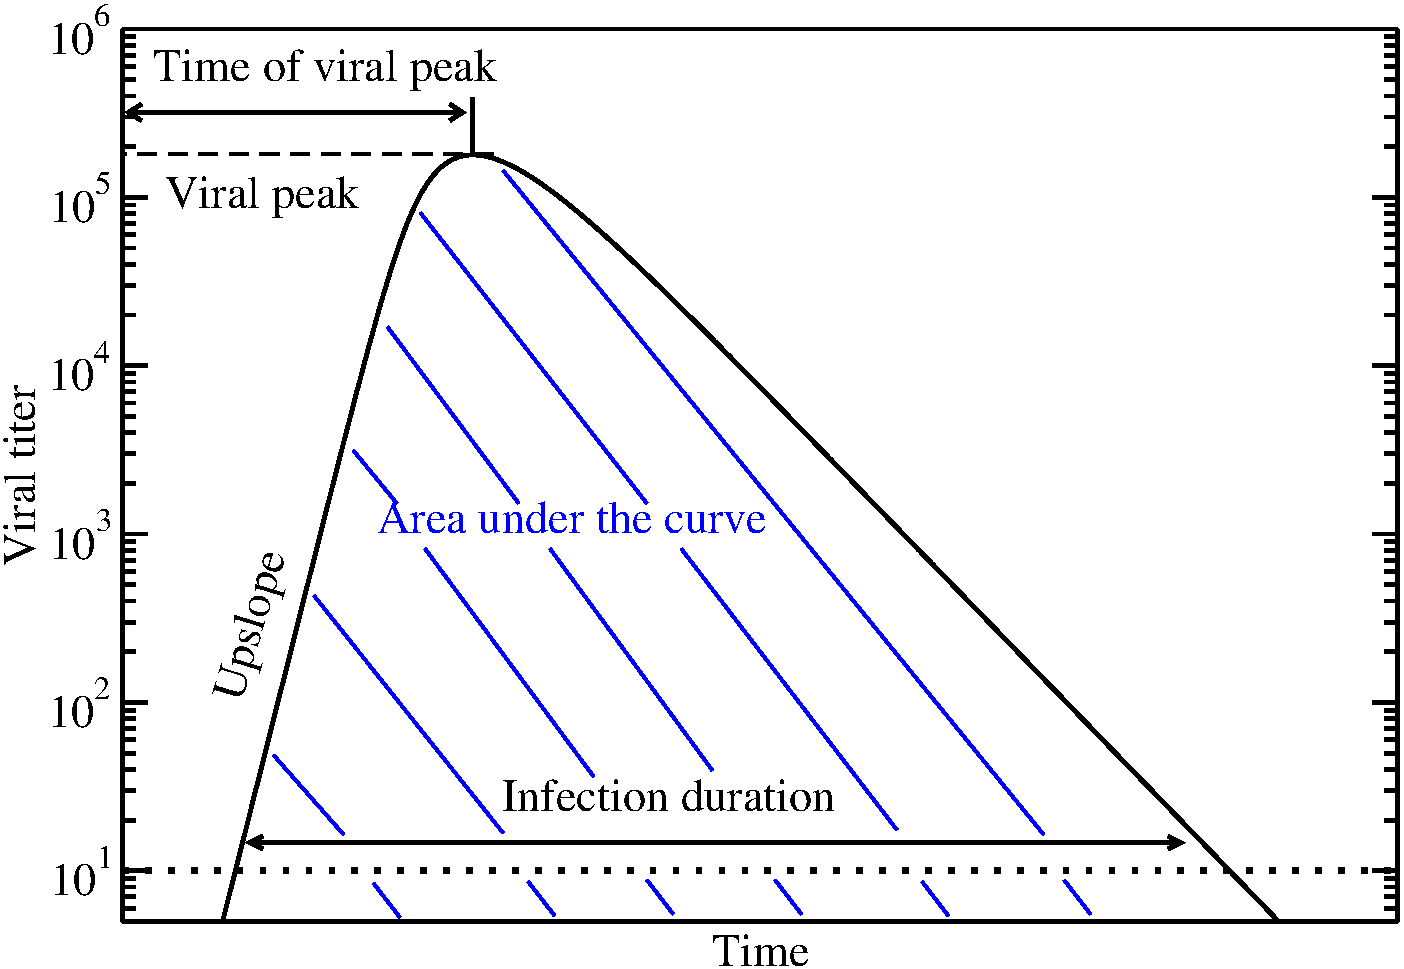
\includegraphics{Figures/measurements}}
\caption{Characteristics of the viral titer curve that are used to assess severity of the infection.\label{measurements}}
\end{center}
\end{figure} 


\section{Results}

Fig.\ \ref{curves} shows the viral titer curves for different MOI of SARS-CoV-2, where the darker line for each color shows the curve of median values and the lighter colored lines are the 100 individual simulations. Note that for most MOI, there is very little variation between simulations once the viral titer is large. The exception is the lowest MOI of 10$^{-5}$ where there is more variation in the exact trajectory of the viral load. We see some obvious shifts in the viral titer curve as the MOI increases. For high MOI, the viral titer curve reaches its peak very quickly, with lower MOIs moving the peak farther out in time. The peak also becomes broader and lower as the MOI becomes lower, suggesting longer infection durations, but with lower viral loads.
\begin{figure}[!h]
\begin{center}
\resizebox{0.6\textwidth}{!}{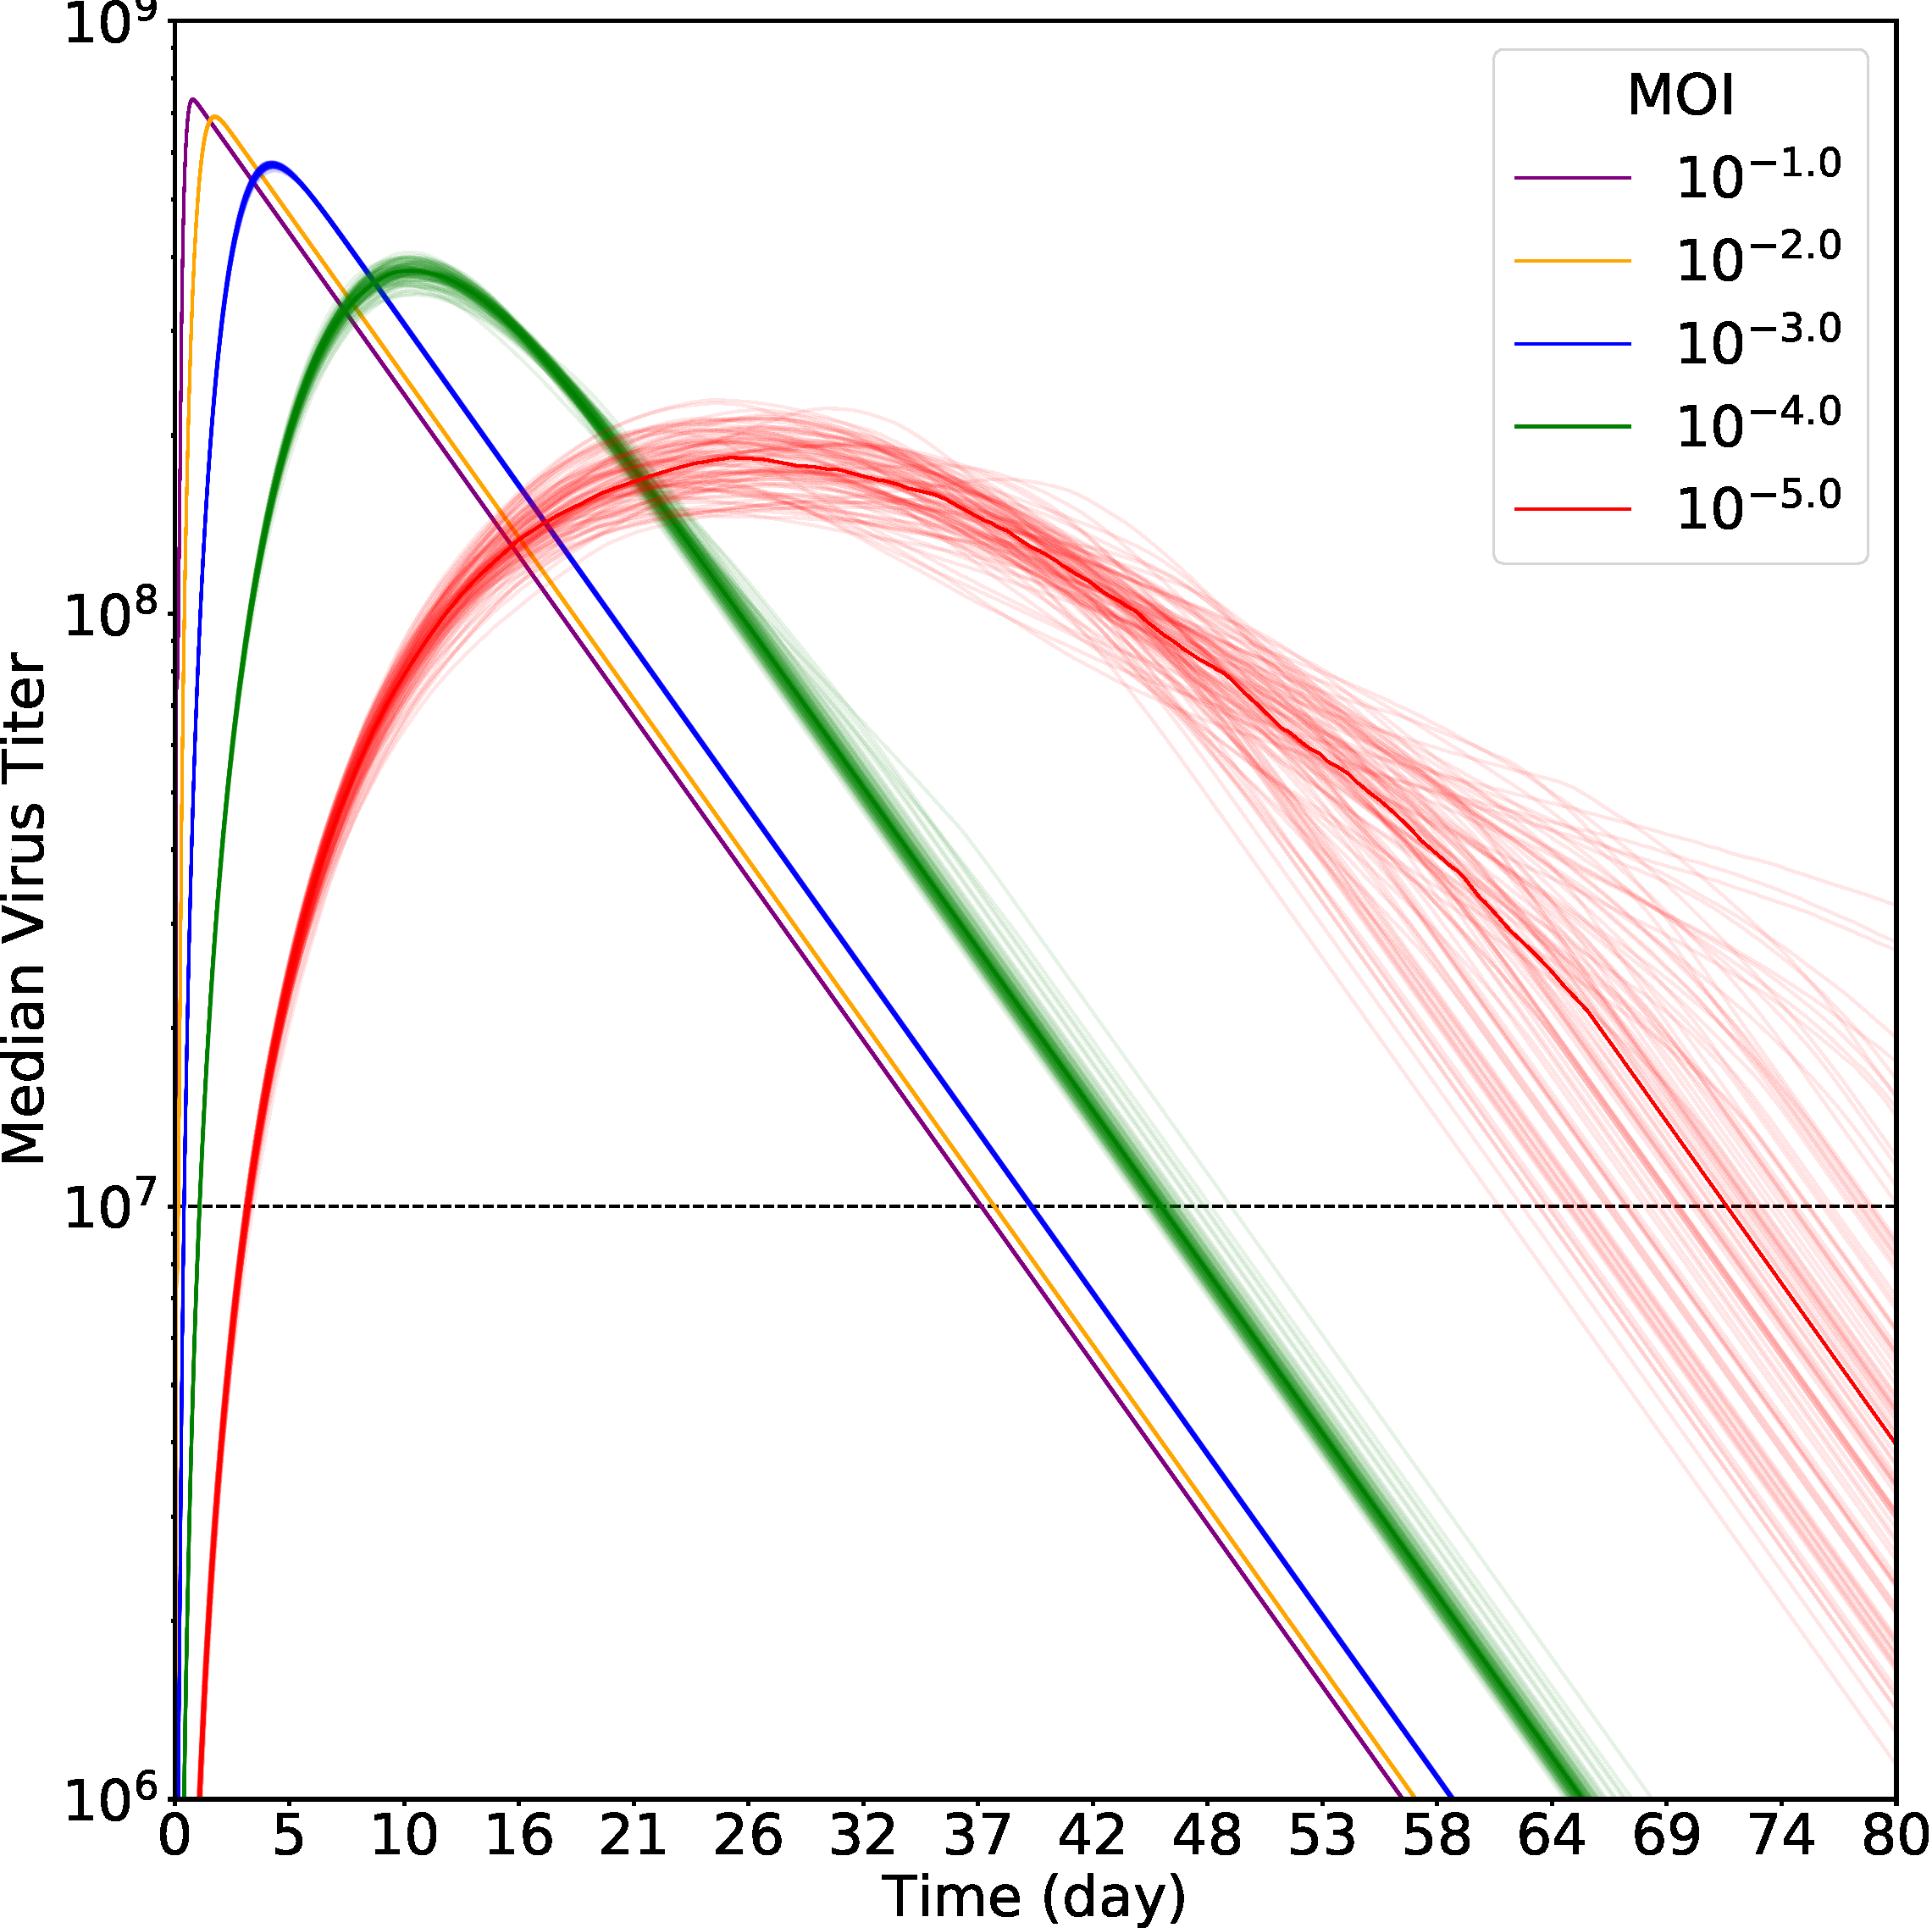
\includegraphics{Figures/Covid_AllOnOne_Median_VirusVsTime}}
\caption{Viral loads for infections initiated with different MOI. Dark lines of each color indicate the viral load curve using the median of 100 simulations, while the lighter colored lines show the viral load kinetics for each individual simulation. The dashed line indicates the threshold of detection used to calculate infection duration. \label{curves}}
\end{center}
\end{figure}

For a more quantitative assessment, we measure the characteristics described in Methods. The results are shown in Fig.\ \ref{results}, which shows peak viral load (top left), time of viral peak (top right), viral upslope (center left), AUC (center right), and infection duration (bottom) as functions of the MOI. The peak viral load increases with increasing initial inoculum, but it appears to reach a plateau as we near an MOI of 1. The time of peak, on the other hand, decreases with increasing initial inoculum, reaching a fixed small value at high MOI. There are real plateaus here since each cell will produce an average of $p\tau_I$ viral particles. At an MOI of 1, all cells are initially infected and will start producing virus at about the same time, meaning that all that virus is released almost simultaneously and there is no second cycle of infection. At slightly lower MOIs, most cells are initially infected, but some cells will be infected in a second or third cycle of infection, reducing the large burst of virus at one time, which causes a delay, reduction, and broadening in the peak. The upslope, or growth rate, of the viral titer curve increases as the MOI increases. This is also driven by the larger amount of virus being produced in the first cycle of infection as the MOI increases. Finally, the AUC and infection duration both decrease as the initial inoculum increases.  
\begin{figure}[!h]
\begin{center}
%\resizebox{0.48\textwidth}{!}{\includegraphics{Figures/CovidApectGraphs/PeakViralTitter}}
%\resizebox{0.48\textwidth}{!}{\includegraphics{Figures/CovidApectGraphs/TimeofPeakViralTitter}}
%\resizebox{0.48\textwidth}{!}{\includegraphics{Figures/CovidApectGraphs/New_UpSlope}}
%\resizebox{0.48\textwidth}{!}{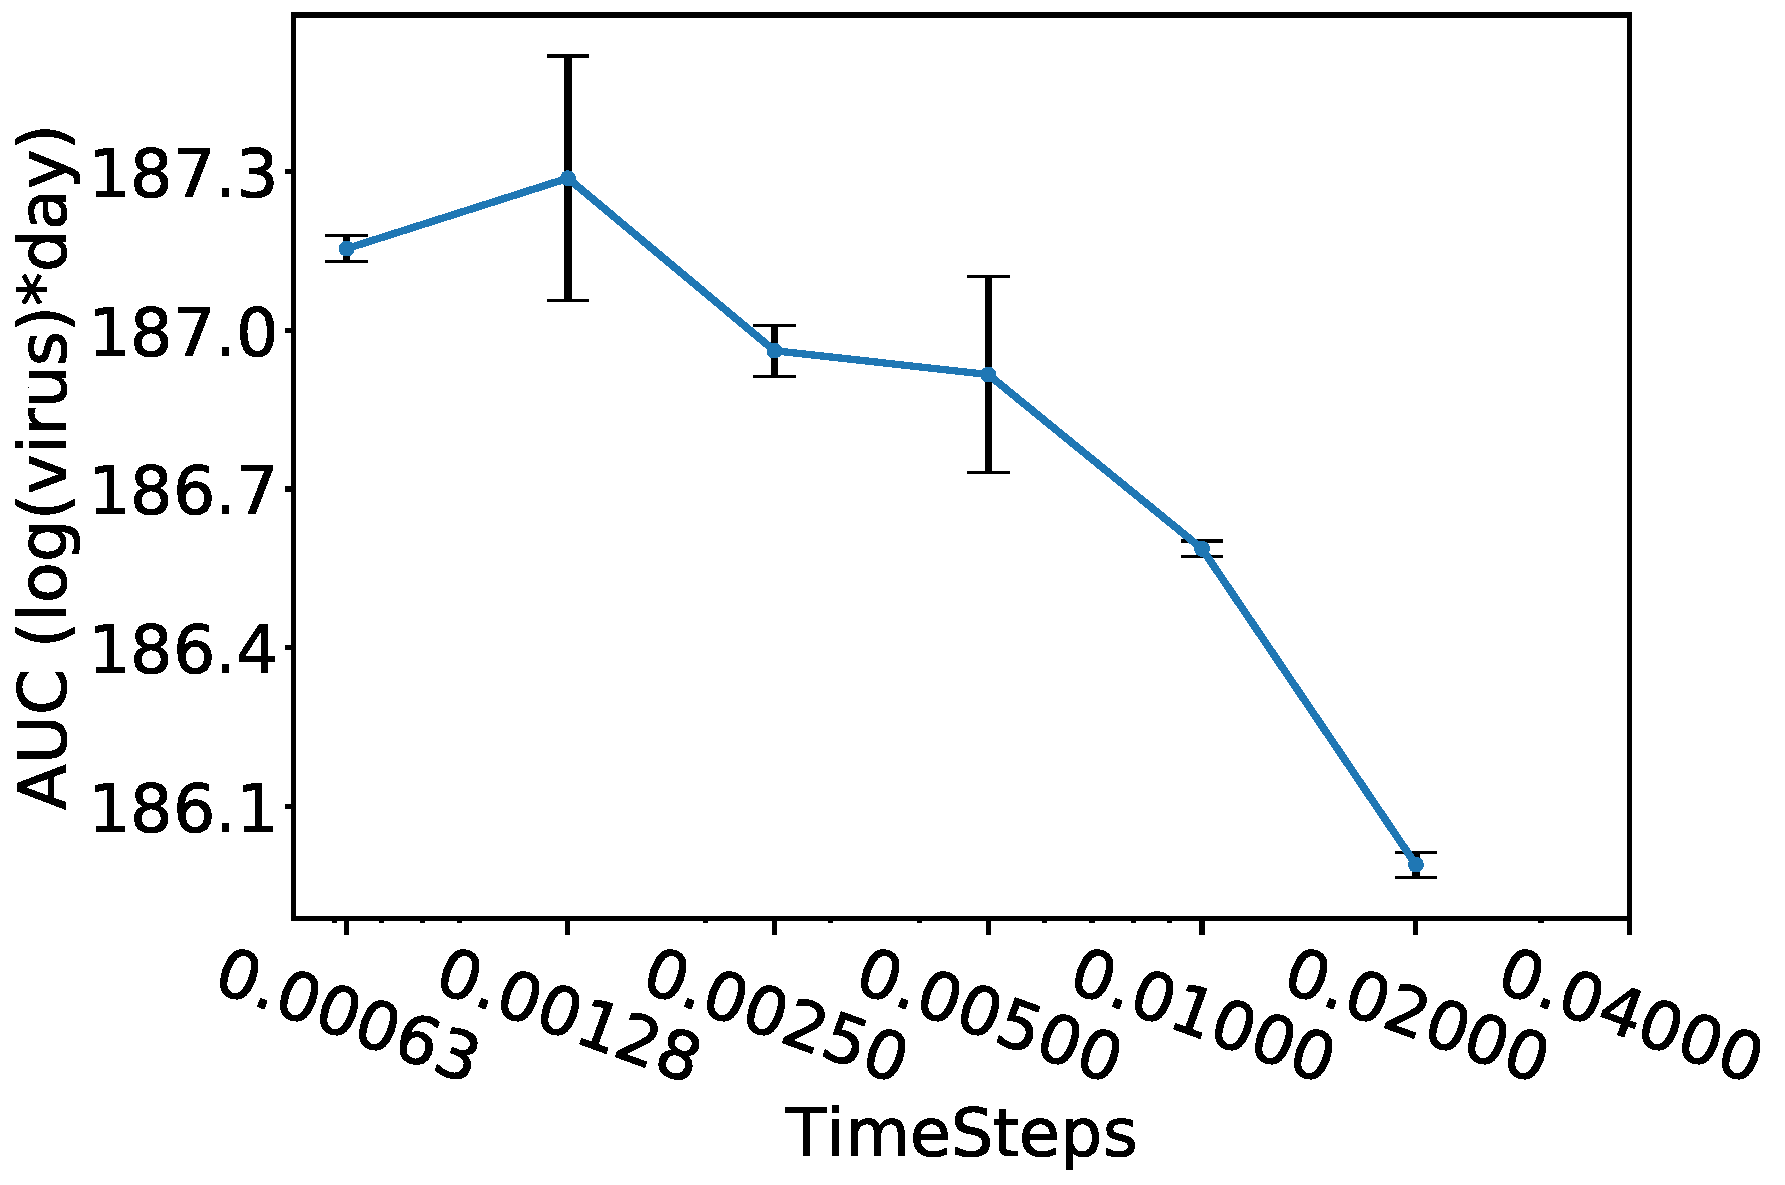
\includegraphics{Figures/CovidApectGraphs/AUC}}
%\resizebox{0.48\textwidth}{!}{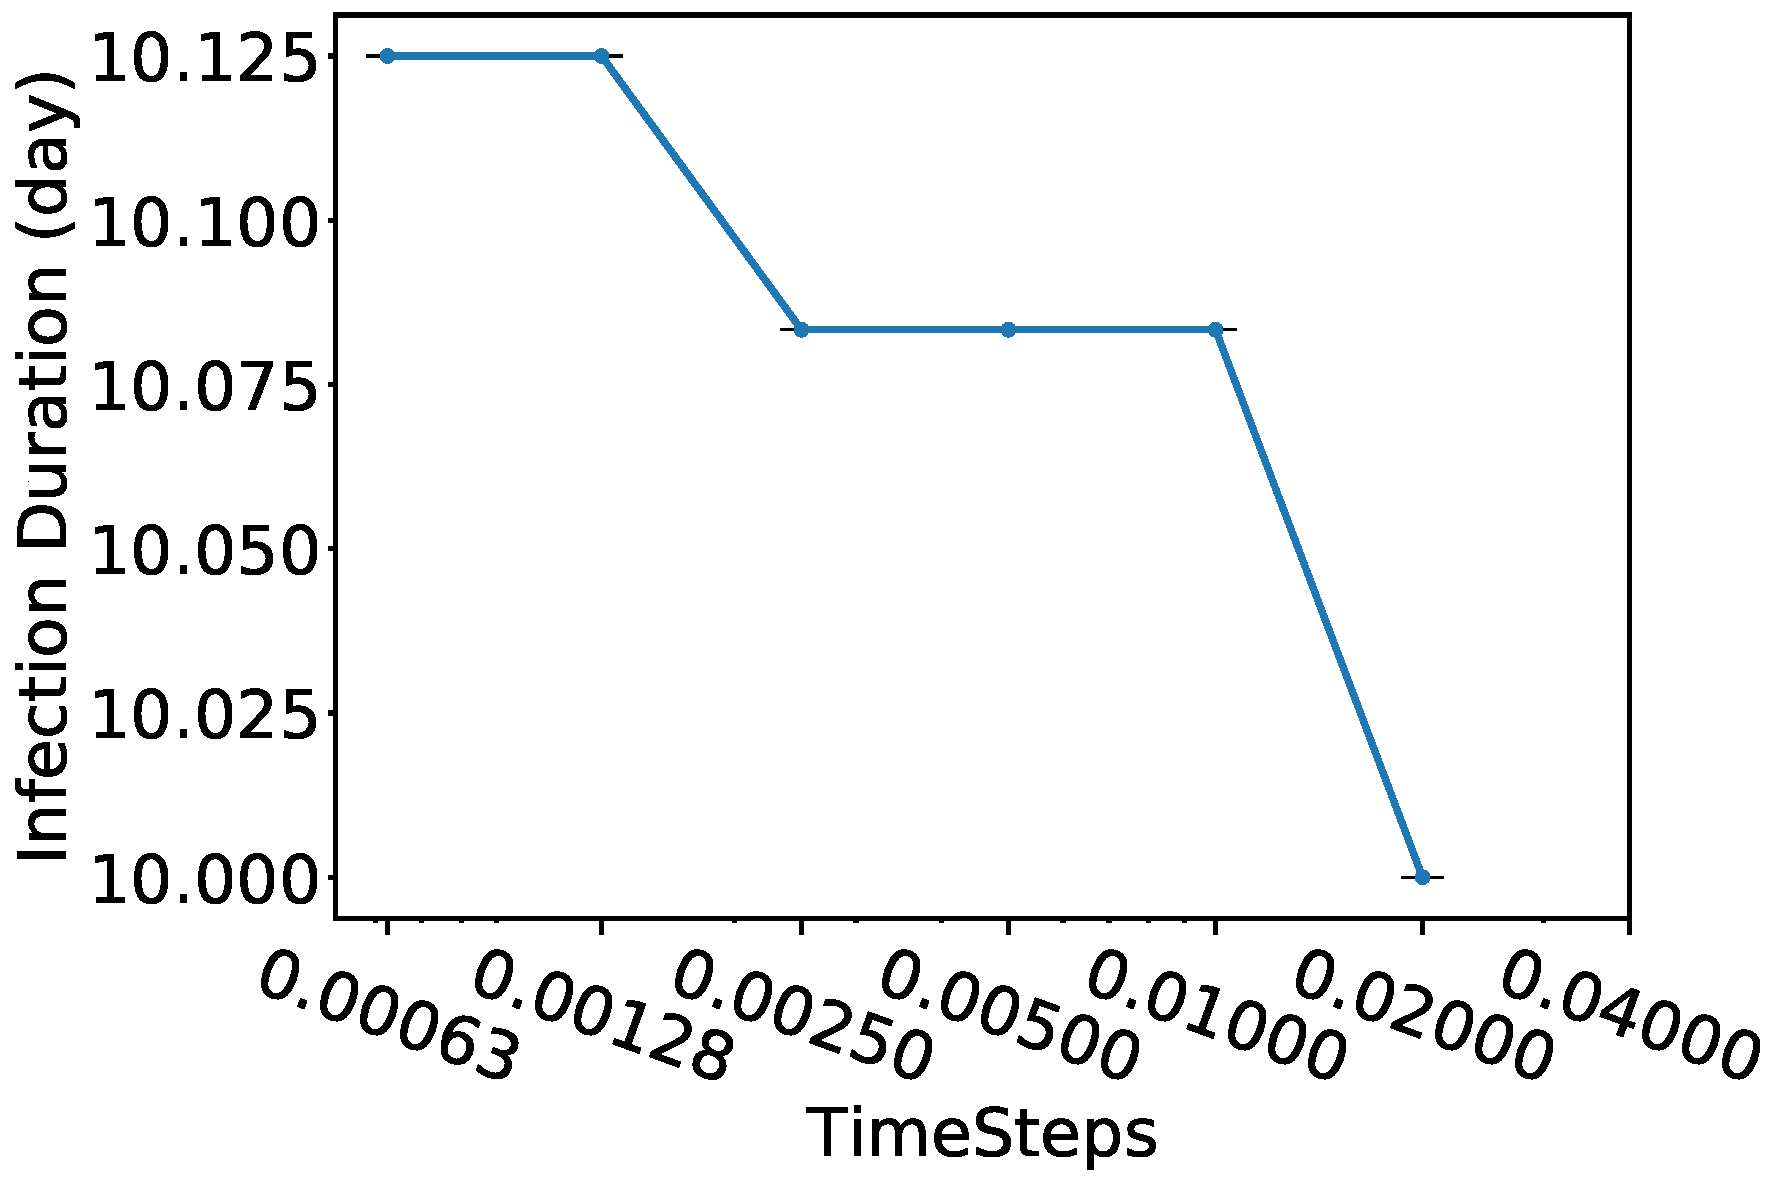
\includegraphics{Figures/CovidApectGraphs/InfectionDuration}}
\caption{Effect of initial inoculum on viral titer characteristics. The graphs show peak viral load (top left), time of viral peak (top right), viral upslope (center left), AUC (center right), and infection duration (bottom) as functions of MOI. \label{results}}
\end{center}
\end{figure}

%%%%%%%%%%%%%%%%%%%%%%%%%%%%%%%%%%%%%%%%%%
\section{Discussion}

Our study finds that initial viral inoculum does alter the viral time course by increasing the peak viral load, moving the peak earlier, increasing the viral upslope, and decreasing both AUC and infection duration, as the initial inoculum increases. 



\chapter{Discussion}
In the previous chapter the model as applied to SARS-CoV-2 data and shown how the model can be used to study the virus. In this chapter, the findings, extensions of the model, and future work of this thesis will be discussed. I will discuss how the proposed model forms a foundation for future work, how the model will be extended with more cellular processes, and how the application of the model gives insight to disease severity.

\section{Findings}

This paper shows that the use of GPUs to accelerate computation of agent-based and partial-differential equation hybrid models allows for simulation results within hours, but with the necessary level of detail to capture individual cell effects, and allows for parameterizing the model quickly. The model in this work accurately replicates the diffusion of a virus, the stages of infection of individual cells, and can be fit to data within hours. While still lacking some of the biology needed for replication of \emph{in vivo} infections, the speed of computation leaves room for incorporation of additional features. Thus, this model implementation forms the foundation of a modeling and simulation tool that can accurately predict in-host viral dynamics and be quickly deployed to help combat the next pandemic.

\section{Model extensions}

Although our model currently only incorporates cell-free transmission, since the ABM models interactions of each cell in a culture dish, the spatial aspects of different viral transmission routes can be explored in detail. There has been recent interest in viruses that transmit via cell to cell transmission, with ODE \citep{allen15,komarova13,iwami15}, stochastic \citep{graw15}, and ABM \citep{kumberger18,blahut21} models developed to study how cell to cell transmission alters infection dynamics. There are also viruses that cause cells that form syncytia, which are cells that have fused into a single multi-nucleated cell. Not much is known about how syncytia alter infection dynamics, with a recent ODE model attempting to assess the effect of syncytia on viral time course \citep{jessie21}, but spatial effects really need to be included for a proper assessment of the role of syncytia. Finally, advection can be added to the diffusion of the virus particles to more closely mimic the respiratory tract. Recent PDE \citep{quirouette20} and ODE \citep{gonzalez19} models both indicate that the addition of advection can limit the spread of respiratory viruses towards the lower respiratory tract, but the stochasticity included in an ABM might affect this result. 

While the model is able to replicate a typical viral time course during an infection, it is missing many components that play important roles in the infection. For example, the immune response of the host has not been added to the model. The immune response is a large, if not the main, contributing factor to symptoms experienced during a viral infection \citep{manchanda14,zheng18}, but also limits spread of infection itself \citep{dobrovolny13}. ABMs are already used to model various aspects of the immune response \citep{whitman20,kerepesi19,levin16}, so the immune response can be incorporated into the existing ABM/PDM framework. Cell tropism, the preference of virus for one cell type over another, is another feature of viral infections that can be incorporated into the ABM. ODE modeling indicates that cell tropism can lead to longer lasting infections \citep{dobrovolny10}, but will also likely affect the spatial dynamics of infection. Finally, variation in production of virus by individual cells \citep{timm12} can be incorporated to determine how this type of cell heterogeneity affects spatiotemporal infection dynamics.

%%%%%%%%%%%%%%%%%%%%%%%%%%%%%%%%%%%%%%%%%%%%%%%%%%%%%%%%%%%%%%%%%%%%%%%%%%%%%%%%%%%%%

\section{Application to disease severity}

The model was used to study the effect of initial viral inoculum on viral time course, finding that increasing inoculum increased the peak viral load, moved the peak earlier, increased the viral upslope, and decreased both AUC and infection duration. It is not immediately clear what these changes in viral kinetics mean for the severity of the infection. Is it better to have a shorter infection, albeit with a higher viral peak, or a longer-lasting infection with a lower viral burden? One study compared viral loads in patients with mild and severe illness finding that the viral load time course in mild cases peaked earlier and at a lower peak viral load than in severe cases, although both time courses still had rather high viral loads at 25 days post symptom onset \citep{zheng20}. Since viral load in these patients was measured after they presented at a hospital, there is also no way to link particular features of the viral time course to the initial inoculum. Other observational studies that have attempted to investigate links between viral load and disease severity have taken a limited number of viral load measurements, often well after the peak of the infection \citep{liu20, liu20imm,to20}, making it impossible to assess the full time course of the viral load, and any correlations to initial inoculum. An alternative to observational studies in patients is to investigate inoculum dose-response of SARS-CoV-2 in animals, as suggested in \citep{little20}. Such animal studies in conjunction with mathematical modeling studies will help provide a clearer picture of the role of initial inoculum in determining viral time course and disease severity.

Infection durations were found to range from 37--73 days. Studies suggest that median duration of viral shedding is 14--20 days after symptom onset, with some patients shedding virus for more than 30 days after symptom onset \citep{qi20, he20shed, zhou20, lee20}. One Italian study found a longer median shedding duration of 36 days after symptom onset \citep{mancuso20}. There are, however, cases of patients who have shed virus for longer periods of time, with several case studies finding patients who shed virus for more than 60 days after hospitalization \citep{park20, liu20, li20shed}. In some studies, longer duration of viral shedding is associated with more serious clinical outcomes such as ICU admission or invasive ventilation \citep{zeng20, lee20}, although other studies have noted that asymptomatic patients also seem to shed virus for longer than mildly symptomatic patients \citep{long20}.

Our findings indicating a decrease in AUC, but an increase in viral peak as MOI increases could be viewed as contradictory since both peak viral load and AUC are supposed to be indicators of disease severity. However, disease severity is often ill-defined. One study has shown a correlation between viral load and total symptom score \citep{chen12} and another between nasal discharge and viral load \citep{handel15} for influenza. This implies that a higher peak viral load should lead to higher symptom score, at least around the time of viral peak. Clinical studies, however, tend to use area under the viral curve as an endpoint in studies as an indicator of disease severity \citep{devincenzo20, hershberger19, stevens18, devincenzo15}, perhaps in an attempt to combine both the severity of symptoms and the duration over which symptoms are experienced. This leads back to the question of whether severity should be assessed by the worst period of symptoms, even it is only for a short duration, or whether disease severity should be assessed by milder, but sustained, symptoms.

Viral load on its own is not the only cause of the symptoms experienced by patients. The immune response is thought to underlie many of the symptoms that cause patient discomfort \citep{hijano19} and medical complications \citep{xu19} for other respiratory viruses. A study using the coronavirus that causes Middle East respiratory syndrome found that high viral load was correlated to high levels of inflammatory cytokines that are, in turn, linked to higher mortality \citep{alosaimi20}. Several studies also hypothesize a connection between intensity of the immune response and severe disease for SARS-CoV-2 \citep{lin20,cao20path,zhu20cardio}. For other respiratory infections, there are several studies that link the size of viral inoculum to variations in various components of the immune response \citep{go19, littwitz17, handel18, redeker14, anderson10}. Another study links area under neutrophils curve and area under IL-8 curve to symptom severity in respiratory tract infections \citep{henriquez15}. Unfortunately, our model does not include an immune response, and so cannot investigate how immune response might vary with initial inoculum dose and affect the severity of the infection. While mathematical models that include immune responses \citep{dobrovolny13} and symptoms \citep{canini11,price15} have been examined for other respiratory viral infections, there is currently not enough time course data on SARS-CoV-2 immune responses to properly assess the validity of these models for the novel coronavirus.  

There are other factors that affect whether a large exposure will lead to severe infection. Simulations show that the site of deposition within the respiratory tract affects not only whether an infection takes hold, but also how easily the virus will replicate \citep{haghnegahdar19}. Like other respiratory viruses, SARS-CoV-2 tends to result in more severe infections when it manages to extend to the lower respiratory tract \citep{COVID20}. The ability to spread to the lower respiratory tract seems to be related to mucosal velocity within the respiratory tract \citep{gonzalez19,quirouette20}, and not directly to viral replication, so this is yet another factor that needs to be considered in determining the severity of the infection. Since our model does not spatially reproduce the respiratory tract, factors that might alter our predictions of viral time course cannot be assessed.

The model used here is fairly generic and simulates SARS-CoV-2 only through choice of parameters. However, the effect of initial inoculum on viral titer has not previously been examined in an ABM of viral dynamics. Previous studies using ordinary differential equation (ODE) models suggest that model structure and underlying assumptions change the predicted dose-response \citep{wethington19, li14}. Interestingly, the ABM is target-cell limited, and draws its parameter values from a fit of a target-cell limited model to SARS-CoV-2 data, but the dose-response trends observed here are quite different from the dose response trends observed with a traditional target-cell limited ODE model \citep{wethington19,li14}. For example, in the target-cell limited ODE, viral titer peak and growth rate do not change with initial inoculum \citep{wethington19, li14}, but the ABM predicts an increase in both. Time of viral peak and infection duration trends for the ABM are similar to those predicted by target-cell limited ODEs \citep{wethington19, li14}.

\section{Future Work}
\section{Conclusion}



\appendix   % Use \input statements to include any necessary appendices
blank


\backmatter 
\bibliography{allbibliographies}
\vita{TextBlock/vita}  % Document which contains the text or tabular with your vita information
\abstract{TextBlock/abstract}  % Document which contains the text of your abstract

\end{document}
